\documentclass[10pt,a4paper]{article}
\usepackage[margin=18mm,top=22mm,bottom=18mm,headsep=7mm,footskip=9mm]{geometry}
\usepackage{fontspec,amsmath,amssymb,array,tabularx,xcolor,tikz,fancyhdr,hyperref}
\usetikzlibrary{arrows.meta}
\setmainfont{NotoSansKR-Regular.ttf}[Path=../../assets/fonts/,BoldFont=NotoSansKR-Semibold.ttf]
\newfontfamily\brandfont{NotoSansKR-Regular.ttf}[Path=../../assets/fonts/,BoldFont=NotoSansKR-Semibold.ttf]
\XeTeXlinebreaklocale "ko"
\XeTeXlinebreakskip=0pt plus 1pt
\definecolor{ink}{HTML}{25343D}
\definecolor{accent}{HTML}{216B7A}
\definecolor{muted}{HTML}{637078}
\definecolor{grid}{HTML}{D9E0E3}
\definecolor{soft}{HTML}{F2F6F6}
\definecolor{vectorblue}{HTML}{266CA8}
\definecolor{vectorteal}{HTML}{278276}
\definecolor{answerred}{HTML}{C42030}
\newif\ifanswers
\answerstrue
\hypersetup{colorlinks=true,urlcolor=accent,pdftitle={OZ Lab AI Study: Linear Algebra Visual Quiz Answer Key},pdfauthor={OZ Lab}}
\setlength{\parindent}{0pt}
\setlength{\parskip}{2pt}
\setlength{\headheight}{21pt}
\setlength{\tabcolsep}{3pt}
\renewcommand{\arraystretch}{1.25}
\pagestyle{fancy}\fancyhf{}
\fancyhead[L]{\brandfont\fontsize{8}{10}\selectfont\bfseries\color{ink}OZ Lab\quad AI Study}
\fancyhead[R]{\brandfont\fontsize{7.5}{10}\selectfont\color{muted}Linear Algebra\quad /\quad Visual Check}
\fancyfoot[L]{\brandfont\fontsize{7}{9}\selectfont\color{muted}3BLUE1BROWN\quad /\quad ESSENCE OF LINEAR ALGEBRA}
\fancyfoot[R]{\brandfont\fontsize{8}{10}\selectfont\color{ink}0\thepage\quad{\color{muted}/\ 03}}
\renewcommand{\headrulewidth}{.3pt}
\renewcommand{\headrule}{\hbox to\headwidth{\color{grid}\leaders\hrule height\headrulewidth\hfill}}
\newcommand{\vc}[2]{\begingroup\renewcommand{\arraystretch}{1}\begin{bmatrix}#1\\#2\end{bmatrix}\endgroup}
\newcommand{\mat}[4]{\begingroup\renewcommand{\arraystretch}{1}\begin{bmatrix}#1&#2\\#3&#4\end{bmatrix}\endgroup}
\newcommand{\sect}[2]{\par\vspace{3mm}{\brandfont\fontsize{10}{15}\selectfont\bfseries\color{accent}#1}\quad{\fontsize{14}{18}\selectfont\bfseries\color{ink}#2}\par\vspace{3mm}}
\newcommand{\q}[2]{\par\noindent\makebox[7mm][l]{\brandfont\fontsize{10}{14}\selectfont\bfseries\color{accent}#1}\begin{minipage}[t]{\dimexpr\linewidth-7mm}\fontsize{9.5}{14}\selectfont #2\end{minipage}\par\vspace{1mm}}
\newcommand{\given}[1]{\par\hspace*{7mm}{\fontsize{10}{15}\selectfont$\displaystyle #1$}\par\vspace{1mm}}
\newcommand{\opt}[3]{{\leavevmode\ifanswers\ifnum#1=#2\color{answerred}\fi\fi(#1)\enspace #3}}
\newcommand{\choices}[5]{\par\hspace*{7mm}\begin{minipage}{\dimexpr\linewidth-7mm}\fontsize{9}{13}\selectfont\begin{tabularx}{\linewidth}{@{}X X@{}}\opt{1}{#1}{#2}&\opt{2}{#1}{#3}\\[4mm]\opt{3}{#1}{#4}&\opt{4}{#1}{#5}\end{tabularx}\end{minipage}\par}
\newcommand{\stackchoices}[5]{\par\hspace*{7mm}\begin{minipage}{\dimexpr\linewidth-7mm}\fontsize{9}{13.5}\selectfont{\opt{1}{#1}{#2}}\par{\opt{2}{#1}{#3}}\par{\opt{3}{#1}{#4}}\par{\opt{4}{#1}{#5}}\end{minipage}\par}
\newcommand{\solution}[2]{\par\vspace{1mm}\hspace*{7mm}\begin{minipage}[t][#1][t]{\dimexpr\linewidth-7mm}\vspace{0pt}\fontsize{8.3}{12}\selectfont\ifanswers\leavevmode\color{answerred}#2\else{\color{grid}\hrule height .3pt}\fi\end{minipage}\par}
\newcommand{\sep}{\vspace{3mm}{\color{grid}\hrule height .25pt}\vspace{3mm}}
\newcommand{\smallaxes}{
  \draw[grid,line width=.2pt,step=1] (-2,-2) grid (2,2);
  \draw[-{Stealth[length=1.4mm]},ink,line width=.4pt] (-2.25,0)--(2.25,0);
  \draw[-{Stealth[length=1.4mm]},ink,line width=.4pt] (0,-2.25)--(0,2.25);
}
\newcommand{\spanplot}[1]{\begin{tikzpicture}[x=.62cm,y=.62cm,baseline=(current bounding box.center)]
  \path[use as bounding box] (-2.45,-2.45) rectangle (2.45,2.45);
  \ifnum#1=1\fill[accent!12] (-2,-2) rectangle (2,2);\fi
  \smallaxes
  \ifnum#1=2\draw[-{Stealth[length=2mm]},accent,line width=1pt] (0,0)--(2.15,2.15);\fill[accent] (0,0) circle(1.4pt);\fi
  \ifnum#1=3\draw[accent,line width=1pt] (0,0)--(1.6,1.6);\fill[accent] (0,0) circle(1.4pt);\fill[accent] (1.6,1.6) circle(1.4pt);\fi
  \ifnum#1=4\draw[{Stealth[length=2mm]}-{Stealth[length=2mm]},accent,line width=1pt] (-2.15,-2.15)--(2.15,2.15);\fi
  \ifanswers\ifnum#1=4\draw[answerred,line width=.8pt] (-2.4,-2.4) rectangle (2.4,2.4);\fi\fi
\end{tikzpicture}}
\AtBeginDocument{\fontsize{9.5}{14}\selectfont\color{ink}}
\begin{document}

{\brandfont\fontsize{19}{24}\selectfont\bfseries Linear Algebra\par}
\vspace{1mm}
{\fontsize{11}{16}\selectfont 벡터에서 행렬과 내적까지}\hfill{\ifanswers\color{answerred}\bfseries 정답 및 해설\else\color{muted}개념 확인\fi}\par
\vspace{3mm}
{\fontsize{8}{12}\selectfont\color{muted}이름\quad\rule{34mm}{.3pt}\hfill 날짜\quad\rule{28mm}{.3pt}}\par
\vspace{2mm}
{\fontsize{8}{12}\selectfont\color{muted}각 문항에서 답 하나를 고르시오\quad ·\quad 계산과 작도는 여백에 해보시오\quad ·\quad 25분}
\sect{01}{벡터와 Span}

\q{1}{행렬 계산과 함께 \textbf{공간이 변하는 모습}을 이해하려는 이유로 가장 적절한 것을 고르시오}
\stackchoices{2}
{그림이 있으면 정확한 수치 계산은 항상 생략할 수 있음}
{계산의 의미를 해석하고, 어떤 연산이 필요한지 판단할 수 있음}
{모든 행렬이 벡터를 회전시키는 같은 연산임을 확인할 수 있음}
{기하학적 의미는 수치 계산과 별개이므로 따로 외울 수 있음}
\solution{10mm}{정답 (2)\quad 숫자 계산은 결과를 구하고, 기하학적 해석은 연산의 의미와 쓰임을 이해하는 데 도움을 줌}
\sep

\q{2}{$\mathbf r=2\mathbf u-\mathbf v$를 \textbf{계산하고 격자에 그려보시오}\quad $\mathbf r$의 좌표를 고르시오}
\begin{minipage}[t]{.59\linewidth}
\given{\mathbf u=\vc{1}{2},\qquad \mathbf v=\vc{-1}{1}}
\vspace{2mm}
\choices{3}{$\vc{1}{3}$}{$\vc{3}{5}$}{$\vc{3}{3}$}{$\vc{1}{5}$}
\vspace{2mm}
\solution{19mm}{정답 (3)\quad $2\mathbf u-\mathbf v=(2,4)-(-1,1)=(3,3)$\\음수를 빼면 양수를 더하는 것과 같음}
\end{minipage}\hfill
\begin{minipage}[t]{.37\linewidth}\vspace{0pt}\centering
\begin{tikzpicture}[x=.62cm,y=.62cm]
\path[use as bounding box] (-2.7,-1.5) rectangle (4.7,5.4);
\draw[grid,line width=.25pt,step=1] (-2,-1) grid (4,5);
\draw[-{Stealth[length=1.7mm]},line width=.5pt] (-2.3,0)--(4.35,0) node[right]{\scriptsize$x$};
\draw[-{Stealth[length=1.7mm]},line width=.5pt] (0,-1.2)--(0,5.2) node[above]{\scriptsize$y$};
\foreach \x in {-2,1,2,3,4}{\node[below,fill=white,inner sep=.7pt] at (\x,0){\tiny$\x$};}
\foreach \y in {1,2,3,4,5}{\node[left,fill=white,inner sep=.7pt] at (0,\y){\tiny$\y$};}
\node[below left] at (0,0){\tiny$0$};
\draw[-{Stealth[length=2mm]},vectorblue,line width=1pt] (0,0)--(1,2) node[above right]{\small$\mathbf u$};
\draw[-{Stealth[length=2mm]},vectorteal,line width=1pt] (0,0)--(-1,1) node[above left]{\small$\mathbf v$};
\ifanswers
\draw[dashed,answerred!65,line width=.65pt] (1,2)--(2,4)--(3,3);
\draw[-{Stealth[length=2mm]},answerred,line width=1pt] (0,0)--(3,3);
\fill[answerred] (3,3) circle(1.6pt);
\node[answerred,above right,fill=white,inner sep=1pt] at (3,3){\scriptsize$\mathbf r$};
\fi
\end{tikzpicture}
\end{minipage}
\sep

\q{3}{$a,b$를 \textbf{모든 실수}로 바꿀 때 만들 수 있는 벡터들의 끝점 전체를 고르시오}
\given{\mathbf u=\vc{1}{1},\quad\mathbf v=\vc{2}{2},\qquad \operatorname{Span}(\mathbf u,\mathbf v)=\{a\mathbf u+b\mathbf v\mid a,b\in\mathbb R\}}
\vspace{2mm}
\begin{tabularx}{\linewidth}{@{}*{4}{>{\centering\arraybackslash}X}@{}}
\spanplot{1}&\spanplot{2}&\spanplot{3}&\spanplot{4}\\
{\fontsize{8.5}{12}\selectfont\opt{1}{4}{평면 전체}}&{\fontsize{8.5}{12}\selectfont\opt{2}{4}{양의 방향 반직선}}&{\fontsize{8.5}{12}\selectfont\opt{3}{4}{두 점 사이 선분}}&{\fontsize{8.5}{12}\selectfont\opt{4}{4}{양쪽으로 뻗는 직선}}
\end{tabularx}
\solution{14mm}{정답 (4)\quad $\mathbf v=2\mathbf u$이므로 $a\mathbf u+b\mathbf v=(a+2b)\mathbf u$\\음수 배수도 가능하므로 원점을 지나 양쪽으로 뻗는 $y=x$ 전체를 만들 수 있음}

\newpage
\sect{02}{기저와 Linear Transformation}

\q{4}{다음 중 \textbf{평면 전체의 Basis}가 될 수 있는 벡터 묶음을 고르시오}
\choices{1}
{$\vc{1}{0},\ \vc{1}{1}$}
{$\vc{1}{2},\ \vc{2}{4}$}
{$\vc{1}{0},\ \vc{0}{0}$}
{$\vc{1}{0},\ \vc{0}{1},\ \vc{1}{1}$}
\solution{14mm}{정답 (1)\quad 두 벡터가 평행하지 않아 평면 전체를 만들며, 서로 중복되지 않음\\(4)는 평면을 만들지만 세 번째 벡터가 앞의 두 벡터의 합이므로 Basis가 아님}
\sep

\q{5}{다음 중 \textbf{Linear Transformation}을 고르시오}
\given{T(a\mathbf u+b\mathbf v)=aT(\mathbf u)+bT(\mathbf v)}
\choices{3}
{$T(x,y)=(x+1,\ y)$}
{$T(x,y)=(x^2,\ y)$}
{$T(x,y)=(2x,\ x+y)$}
{$T(x,y)=(x,\ |y|)$}
\solution{17mm}{정답 (3)\quad 덧셈과 실수배를 보존함\\(1)은 원점이 이동함\quad (2)는 $x$를 두 배로 하면 $x^2$이 네 배가 됨\\(4)는 $T(0,-1)\ne -T(0,1)$이므로 음수 배수를 보존하지 못함}
\sep

\q{6}{Linear Transformation $T$가 아래와 같이 두 기저 벡터를 옮긴다\quad \textbf{$T$의 행렬 $A$}를 고르시오}
\begin{minipage}[t]{.63\linewidth}
\given{T\!\left(\vc{1}{0}\right)=\vc{1}{1},\qquad T\!\left(\vc{0}{1}\right)=\vc{-1}{2}}
\vspace{2mm}
\choices{2}{$\mat{1}{1}{-1}{2}$}{$\mat{1}{-1}{1}{2}$}{$\mat{-1}{1}{2}{1}$}{$\mat{1}{0}{0}{1}$}
\end{minipage}\hfill
\begin{minipage}[t]{.34\linewidth}\vspace{0pt}\centering
\begin{tikzpicture}[x=.65cm,y=.65cm]
\path[use as bounding box] (-2.5,-1.6) rectangle (4,3.4);
\draw[grid,line width=.25pt,step=1] (-2,-1) grid (3,3);
\draw[-{Stealth[length=1.7mm]},line width=.5pt] (-2.3,0)--(3.5,0) node[right]{\scriptsize$x$};
\draw[-{Stealth[length=1.7mm]},line width=.5pt] (0,-1.3)--(0,3.2) node[above]{\scriptsize$y$};
\foreach \x in {-2,-1,1,2,3}{\node[below,fill=white,inner sep=.7pt] at (\x,0){\tiny$\x$};}
\foreach \y in {1,2,3}{\node[left,fill=white,inner sep=.7pt] at (0,\y){\tiny$\y$};}
\node[below left] at (0,0){\tiny$0$};
\draw[-{Stealth[length=2mm]},vectorblue,line width=1pt] (0,0)--(1,1) node[above right]{\scriptsize$T(\mathbf e_1)$};
\draw[-{Stealth[length=2mm]},vectorteal,line width=1pt] (0,0)--(-1,2) node[above left]{\scriptsize$T(\mathbf e_2)$};
\ifanswers
\draw[-{Stealth[length=2mm]},answerred,line width=1pt] (0,0)--(3,0);
\fill[answerred] (3,0) circle(1.6pt);
\node[answerred,above,fill=white,inner sep=1pt] at (2.5,.12){\scriptsize$T(\mathbf v)$};
\fi
\end{tikzpicture}
\end{minipage}
\solution{10mm}{정답 (2)\quad 첫 번째 열은 $T(\mathbf e_1)$, 두 번째 열은 $T(\mathbf e_2)$\quad $\mathbf e_1=(1,0),\ \mathbf e_2=(0,1)$}
\sep

\q{7}{6번의 $T$에 아래 벡터 $\mathbf v$를 넣었다\quad \textbf{$T(\mathbf v)$를 위 격자에 표시}하고 좌표를 고르시오}
\given{\mathbf v=\vc{2}{-1},\qquad T(\mathbf v)=2T(\mathbf e_1)-T(\mathbf e_2)}
\choices{4}{$\vc{1}{-4}$}{$\vc{1}{0}$}{$\vc{3}{4}$}{$\vc{3}{0}$}
\solution{16mm}{정답 (4)\quad $T(\mathbf v)=2(1,1)-(-1,2)=(3,0)$\\변환 전의 계수 $2,-1$을 변환된 기저 벡터에도 그대로 적용함}

\newpage
\sect{03}{변환의 합성과 Dot Product}

\q{8}{$\mathbf x$에 \textbf{$A$를 먼저, $B$를 나중에} 적용한다\quad 전체 변환의 행렬과 결과가 모두 맞는 것을 고르시오}
\given{A=\mat{1}{1}{0}{1},\qquad B=\mat{0}{-1}{1}{0},\qquad \mathbf x=\vc{1}{1}}
\choices{1}
{$BA$,\quad 결과 $\vc{-1}{2}$}
{$AB$,\quad 결과 $\vc{-1}{2}$}
{$BA$,\quad 결과 $\vc{0}{1}$}
{$AB$,\quad 결과 $\vc{0}{1}$}
\vspace{2mm}
\given{\mathbf x\ \xrightarrow{\ A\ }\ \underbrace{\hspace{22mm}}_{\text{중간 결과}}\ \xrightarrow{\ B\ }\ \underbrace{\hspace{22mm}}_{\text{최종 결과}}}
\solution{14mm}{정답 (1)\quad $A\mathbf x=(2,1)$,\quad $B(A\mathbf x)=(-1,2)$\quad 따라서 전체 행렬은 $BA$\\순서를 바꾸면 $A(B\mathbf x)=(0,1)$로 결과가 달라짐}
\sep

\q{9}{$\mathbf w$의 끝점에서 $\mathbf v$가 놓인 직선으로 \textbf{수선을 그려보시오}\quad 투영의 길이와 내적이 모두 맞는 것을 고르시오}
\begin{minipage}[t]{.59\linewidth}
\given{\mathbf v=\vc{2}{0},\qquad\mathbf w=\vc{3}{2}}
\given{\mathbf v\cdot\mathbf w=v_1w_1+v_2w_2}
\vspace{2mm}
\choices{3}
{투영 길이 $3$,\quad 내적 $3$}
{투영 길이 $2$,\quad 내적 $4$}
{투영 길이 $3$,\quad 내적 $6$}
{투영 길이 $2$,\quad 내적 $6$}
\end{minipage}\hfill
\begin{minipage}[t]{.37\linewidth}\vspace{0pt}\centering
\begin{tikzpicture}[x=.93cm,y=.93cm]
\path[use as bounding box] (-.6,-.8) rectangle (4.2,3.0);
\draw[grid,line width=.25pt,step=1] (0,0) grid (4,2.5);
\draw[-{Stealth[length=1.7mm]},line width=.5pt] (-.25,0)--(4,0) node[right]{\scriptsize$x$};
\draw[-{Stealth[length=1.7mm]},line width=.5pt] (0,-.3)--(0,2.65) node[above]{\scriptsize$y$};
\foreach \x in {1,2,3}{\node[below] at (\x,0){\tiny$\x$};}
\foreach \y in {1,2}{\node[left] at (0,\y){\tiny$\y$};}
\node[below left] at (0,0){\tiny$0$};
\draw[-{Stealth[length=2mm]},vectorblue,line width=1.2pt] (0,0)--(2,0) node[above]{\small$\mathbf v$};
\draw[-{Stealth[length=2mm]},vectorteal,line width=1pt] (0,0)--(3,2) node[above right]{\small$\mathbf w$};
\ifanswers
\draw[dashed,answerred,line width=.8pt] (3,2)--(3,0);
\draw[answerred,line width=.6pt] (2.8,0)--(2.8,.2)--(3,.2);
\fill[answerred] (3,0) circle(1.7pt);
\draw[answerred,{Stealth[length=1.5mm]}-{Stealth[length=1.5mm]}] (0,-.45)--(3,-.45) node[midway,below]{\scriptsize$3$};
\fi
\end{tikzpicture}
\end{minipage}
\solution{13mm}{정답 (3)\quad 투영의 길이는 $3$,\quad $\mathbf v\cdot\mathbf w=2\times3+0\times2=6$\\내적은 여기서 투영 길이에 $\lVert\mathbf v\rVert=2$를 곱한 값이므로, 투영 길이 자체와 다름}
\sep

\q{10}{벡터를 \textbf{숫자 하나로 보내는 선형변환} $L$이 있다\quad $L(\mathbf x)=\mathbf w\cdot\mathbf x$로 나타낼 때, $\mathbf w$와 $L(\mathbf x)$가 모두 맞는 것을 고르시오}
\given{\mathbf x=\vc{3}{1},\qquad L\!\left(\vc{1}{0}\right)=2,\qquad L\!\left(\vc{0}{1}\right)=-1}
\choices{2}
{$\mathbf w=\vc{-1}{2}$,\quad 결과 $-1$}
{$\mathbf w=\vc{2}{-1}$,\quad 결과 $5$}
{$\mathbf w=\vc{2}{-1}$,\quad 결과 $\vc{6}{-1}$}
{$\mathbf w=\vc{2}{1}$,\quad 결과 $7$}
\solution{17mm}{정답 (2)\quad $\mathbf w=(2,-1)$이고 $L(\mathbf x)=2x_1-x_2$이므로 $L(3,1)=6-1=5$\\벡터 $\mathbf w$ 하나로 숫자를 출력하는 선형변환을 표현할 수 있다는 것이 이 예의 Duality\\ML에서 $b=0$인 $f_{\mathbf w}(\mathbf x)=\mathbf w\cdot\mathbf x$도 같은 형태}
\vfill
{\fontsize{6.7}{9.5}\selectfont\color{muted}
학습 범위\quad 3Blue1Brown 영상 6편 · 문제와 그림은 별도 작성\\
\href{https://www.youtube.com/watch?v=ic_hG2M2nG0}{시각적 이해}\quad
\href{https://www.youtube.com/watch?v=ArgTeYVuJUo}{벡터}\quad
\href{https://www.youtube.com/watch?v=2CcCOgDilO8}{선형결합·Span·Basis}\quad
\href{https://www.youtube.com/watch?v=35ESC-g49fY}{선형변환과 행렬}\quad
\href{https://www.youtube.com/watch?v=gXjCxYuEybQ}{변환의 합성}\quad
\href{https://www.youtube.com/watch?v=zSd7jd2HGhM}{내적과 쌍대성}\\
내용 대조\quad
\href{https://github.com/3b1b/captions/blob/main/2016/eola-preview/english/transcript.txt}{공식 도입 자막}\quad
\href{https://www.3blue1brown.com/lessons/vectors/}{Vectors}\quad
\href{https://www.3blue1brown.com/lessons/span/}{Span}\quad
\href{https://www.3blue1brown.com/lessons/linear-transformations/}{Transformations}\quad
\href{https://www.3blue1brown.com/lessons/matrix-multiplication/}{Composition}\quad
\href{https://www.3blue1brown.com/lessons/dot-products/}{Dot Products}}
\end{document}
